% =====================================================================
%  Reporte.tex
%  ========================
%
%
%  Descripción:
%  ------------
%  Reporte breve del proyecto 1 de Matemáticas para la Computación:
%  objetivo, información utilizada, proceso y análisis de resultados
%  de K-SVD aplicado a señales de ECG de MIT-BIH. Cinco páginas como
%  máximo. Las figuras salen de src/Figuras.py y src/Analisis.py.
%
%
%  Metadata:
%  ----------
%   * Author : zxxz6 (Bryan Violante Arriaga)
%   * Version: 1.0.0
%
%
%  History:
%  ------------
%  Author      Date            Description
%  zxxz6       04/10/2026      Coautores y la serie SEE Matrix en referencias
%  zxxz6       04/10/2026      Creation
%
%
% =====================================================================
\documentclass[11pt,letterpaper]{article}

% =====================================================================
%  DATOS DE LA MATERIA
% =====================================================================
\newcommand{\materia}{Matemáticas para la Computación}
\newcommand{\profesor}{Dra. Hayde Peregrina Barreto \\
                       Dr. Luis Villaseñor Pineda}
\newcommand{\periodo}{Otoño 2026}
\newcommand{\alumno}{Bryan Ezequiel Violante Arriaga}

% =====================================================================
%  Preambulo.tex
%  ========================
%
%
%  Descripción:
%  ------------
%  Preámbulo compartido de los apuntes de clase: paquetes, estilo de
%  página, entornos de teorema, las cuatro cajas de color, el estilo de
%  listings y el pseudocódigo en español. Se carga con \input desde
%  cada documento en lugar de copiarlo, para que un arreglo aquí llegue
%  a todas las libretas de una vez.
%
%
%  Considerations:
%  ------------
%  - Se carga con \input y ruta relativa, no con \usepackage, porque
%    \usepackage solo busca en la carpeta del documento y en el árbol
%    de TeX. Un .sty instalado en TEXMFHOME evitaría la ruta, pero vive
%    fuera del repo y una clona nueva no compilaría
%  - Los cuatro datos de la materia se declaran en el documento ANTES
%    del \input. hyperref expande \materia al cargarse, así que si no
%    existe todavía la compilación truena
%  - Cuando la materia la imparte más de un profesor, los nombres van
%    en un solo \profesor separados por \\. La portadilla los imprime
%    dentro de un center, que es donde \\ sí corta renglón. Repetir
%    \newcommand{\profesor} no es opción: truena con "already defined"
%  - algorithmicx no tiene opción de idioma y babel no lo traduce, así
%    que las palabras clave del pseudocódigo se renombran a mano
%  - Los nombres de los entornos van sin acento (\begin{definicion})
%    aunque el rótulo impreso sí lo lleve
%  - babel se carga con es-noshorthands porque en español el " queda
%    activo y se come el texto que le sigue, además de romper listings
%
%
%  Metadata:
%  ----------
%   * Author : zxxz6 (Bryan Violante Arriaga)
%   * Version: 1.7.0
%
%
%  History:
%  ------------
%  Author      Date            Description
%  zxxz6       24/09/2026      Encabezado de una hoja de un ejercicio
%  zxxz6       23/09/2026      Macros de los documentos de soluciones
%  zxxz6       30/08/2026      Macros de lim, limsup y liminf sobre n
%  zxxz6       25/08/2026      Macros de Omega, Theta, o y omega chicas
%  zxxz6       20/08/2026      Cargue pgfplots para graficas de datos
%  zxxz6       20/08/2026      Cargue tikz para diagramas de conjuntos
%  zxxz6       19/08/2026      Documente \profesor con varios nombres
%  zxxz6       19/08/2026      Agregue la caja Idea Random
%  zxxz6       18/08/2026      Creation
%
%
% =====================================================================
%  USO
%  ---
%  \documentclass[11pt,letterpaper]{article}
%  \newcommand{\materia}{...}      % los cuatro datos van arriba
%  \newcommand{\profesor}{...}
%  \newcommand{\periodo}{...}
%  \newcommand{\alumno}{...}
%  \input{../../templates/Preambulo.tex}
%  \begin{document}
%  \portadilla
%
%  Con dos o mas profesores se declara UN solo \profesor y los nombres
%  se separan con \\, uno por renglon:
%
%  \newcommand{\profesor}{Dra. Fulana de Tal \\
%                         Dr. Mengano de Cual}
% =====================================================================


% ==================== IDIOMA Y CODIFICACIÓN ====================
\usepackage[utf8]{inputenc}
\usepackage[T1]{fontenc}
\usepackage[spanish,es-tabla,es-noshorthands]{babel}
\usepackage{lmodern}
\usepackage{microtype}

% ==================== PÁGINA ====================
\usepackage[letterpaper,margin=2.3cm,headheight=14pt]{geometry}
\usepackage{parskip}
\usepackage{fancyhdr}
\usepackage{enumitem}

% ==================== MATEMÁTICAS ====================
\usepackage{amsmath,amssymb,amsthm,mathtools}

% ==================== FIGURAS, TABLAS, CÓDIGO ====================
\usepackage{graphicx}
\usepackage{booktabs}
\usepackage{array}
% float da el especificador [H], que clava una tabla donde se
% escribio. Una traza que LaTeX manda dos paginas adelante deja
% de leerse junto al paso que la produjo
\usepackage{float}
\usepackage{xcolor}
% tikz ya viene arrastrado por tcolorbox[most], pero se carga
% explicito para no depender de ese detalle; la libreria babel
% protege a tikz de los caracteres activos del español
\usepackage{tikz}
\usetikzlibrary{babel}
% pgfplots dibuja graficas de datos (ejes, escalas log) sobre tikz
\usepackage{pgfplots}
\pgfplotsset{compat=1.18}
\usepackage{listings}
\usepackage[ruled,section]{algorithm}
\usepackage{algpseudocode}
\usepackage[most]{tcolorbox}
% soul da \hl, el unico resaltado que parte renglon; \colorbox no
\usepackage{soul}
\usepackage{hyperref}

% =====================================================================
%  ESTILO
% =====================================================================

% --- encabezado y pie de cada página ---
\pagestyle{fancy}
\fancyhf{}
\fancyhead[L]{\small\textsc{\materia}}
\fancyhead[R]{\small\periodo}
\fancyfoot[C]{\small\thepage}
\renewcommand{\headrulewidth}{0.4pt}

% --- enlaces ---
\hypersetup{
  colorlinks=true,
  linkcolor=black,
  urlcolor=blue,
  citecolor=black,
  pdftitle={Apuntes de \materia},
  pdfauthor={\alumno}
}

% --- paleta ---
\definecolor{acento}{HTML}{1F4E79}
\definecolor{fondoIdea}{HTML}{EAF2FB}
\definecolor{fondoOjo}{HTML}{FDF0E6}
\definecolor{fondoPend}{HTML}{F2F0F7}
\definecolor{comentario}{HTML}{5A7D5A}
\definecolor{cadena}{HTML}{A03030}
\definecolor{fondoCodigo}{HTML}{F7F7F7}
\definecolor{fondoResultado}{HTML}{EAF5EC}
\definecolor{marcador}{HTML}{FFF3A3}

% --- entornos de teorema; numeran por sección, o sea por clase ---
\theoremstyle{definition}
\newtheorem{definicion}{Definición}[section]
\newtheorem{ejemplo}[definicion]{Ejemplo}
\newtheorem{ejercicio}[definicion]{Ejercicio}

\theoremstyle{plain}
\newtheorem{teorema}[definicion]{Teorema}
\newtheorem{lema}[definicion]{Lema}
\newtheorem{corolario}[definicion]{Corolario}
\newtheorem{proposicion}[definicion]{Proposición}

\theoremstyle{remark}
\newtheorem*{observacion}{Observación}
\newtheorem*{quick_sum}{Resumen rápido}

% --- cajas de color para lo que se relee antes del examen ---
\newtcolorbox{idea}[1][]{
  colback=fondoIdea, colframe=acento, boxrule=0.6pt,
  arc=2pt, left=6pt, right=6pt, top=5pt, bottom=5pt,
  title={Idea clave}, fonttitle=\bfseries\small, #1
}
\newtcolorbox{ojo}[1][]{
  colback=fondoOjo, colframe=orange!70!black, boxrule=0.6pt,
  arc=2pt, left=6pt, right=6pt, top=5pt, bottom=5pt,
  title={Ojito...}, fonttitle=\bfseries\small, #1
}
\newtcolorbox{pendiente}[1][]{
  colback=fondoPend, colframe=violet!60!black, boxrule=0.6pt,
  arc=2pt, left=6pt, right=6pt, top=5pt, bottom=5pt,
  title={Pendiente por resolver}, fonttitle=\bfseries\small, #1
}
\newtcolorbox{idear}[1][]{
  colback=fondoPend, colframe=pink!60!black, boxrule=0.6pt,
  arc=2pt, left=6pt, right=6pt, top=5pt, bottom=5pt,
  title={Idea Random}, fonttitle=\bfseries\small, #1
}

% --- el resultado al que llego un ejercicio, para que se vea de
%     lejos al hojear la hoja antes del examen ---
\newtcolorbox{resultado}[1][]{
  colback=fondoResultado, colframe=green!45!black, boxrule=0.6pt,
  arc=2pt, left=6pt, right=6pt, top=5pt, bottom=5pt,
  title={Resultado}, fonttitle=\bfseries\small, #1
}

% --- código ---
\lstdefinestyle{codigo}{
  backgroundcolor=\color{fondoCodigo},
  basicstyle=\ttfamily\footnotesize,
  keywordstyle=\color{acento}\bfseries,
  commentstyle=\color{comentario}\itshape,
  stringstyle=\color{cadena},
  numbers=left, numberstyle=\tiny\color{gray}, numbersep=8pt,
  frame=single, rulecolor=\color{gray!40},
  breaklines=true, showstringspaces=false,
  tabsize=4, captionpos=b,
  extendedchars=true, inputencoding=utf8,
  literate={á}{{\'a}}1 {é}{{\'e}}1 {í}{{\'i}}1
           {ó}{{\'o}}1 {ú}{{\'u}}1 {ñ}{{\~n}}1
           {Ü}{{\"U}}1 {ü}{{\"u}}1 {¿}{{?`}}1
           {¡}{{!`}}1
}
\lstset{style=codigo}
\renewcommand{\lstlistingname}{Código}
\renewcommand{\lstlistlistingname}{Índice de código}
% --- pseudocódigo; algorithmicx arma el cuerpo y algorithm el
%     flotante que lo numera y lo pone en el índice. Las palabras
%     clave vienen en inglés de fábrica y babel no las toca, así que
%     se renombran una por una ---
\floatname{algorithm}{Algoritmo}
\renewcommand{\listalgorithmname}{Índice de algoritmos}

\algrenewcommand\algorithmicrequire{\textbf{Entrada:}}
\algrenewcommand\algorithmicensure{\textbf{Salida:}}
\algrenewcommand\algorithmicend{\textbf{fin}}
\algrenewcommand\algorithmicif{\textbf{si}}
\algrenewcommand\algorithmicthen{\textbf{entonces}}
\algrenewcommand\algorithmicelse{\textbf{si no}}
\algrenewcommand\algorithmicfor{\textbf{para}}
\algrenewcommand\algorithmicforall{\textbf{para todo}}
\algrenewcommand\algorithmicdo{\textbf{hacer}}
\algrenewcommand\algorithmicwhile{\textbf{mientras}}
\algrenewcommand\algorithmicrepeat{\textbf{repetir}}
\algrenewcommand\algorithmicuntil{\textbf{hasta que}}
\algrenewcommand\algorithmicloop{\textbf{ciclo}}
\algrenewcommand\algorithmicprocedure{\textbf{procedimiento}}
\algrenewcommand\algorithmicfunction{\textbf{función}}
\algrenewcommand\algorithmicreturn{\textbf{devolver}}
\algrenewcomment[1]{\hfill{\color{comentario}\itshape // #1}}

% Las dos que algorithmicx no trae. El \ del final es obligatorio: sin
% el TeX se come el espacio y sale "hastan-1" en vez de "hasta n-1"
\algnewcommand\Hasta{\textbf{hasta}\ }
\algnewcommand\Intercambiar{\textbf{intercambiar}\ }

% --- abreviaturas que se usan a cada rato ---
\newcommand{\N}{\mathbb{N}}
\newcommand{\Z}{\mathbb{Z}}
\newcommand{\Q}{\mathbb{Q}}
\newcommand{\R}{\mathbb{R}}
\newcommand{\C}{\mathbb{C}}
\newcommand{\abs}[1]{\left\lvert #1 \right\rvert}
\newcommand{\norm}[1]{\left\lVert #1 \right\rVert}
\newcommand{\set}[1]{\left\{ #1 \right\}}
\newcommand{\Ord}[1]{\mathcal{O}\!\left(#1\right)}
% Mayuscula la notacion grande, minuscula la chica
\newcommand{\Omg}[1]{\Omega\!\left(#1\right)}
\newcommand{\Tht}[1]{\Theta\!\left(#1\right)}
\newcommand{\ord}[1]{o\!\left(#1\right)}
\newcommand{\omg}[1]{\omega\!\left(#1\right)}
% Los tres limites sobre n, que salen en cada renglon del criterio
% del cociente para la notacion asintotica
\newcommand{\LM}{\lim_{n \to \infty}}
\newcommand{\LS}{\limsup_{n \to \infty}}
\newcommand{\LI}{\liminf_{n \to \infty}}

% --- encabezado de cada sesión: título a la izquierda, fecha a la
%     derecha. El argumento corto es el que sale en el índice ---
\newcommand{\clase}[2]{%
  \section[#1]{#1 \hfill \normalfont\small\textit{#2}}%
}

% --- portadilla y tabla de contenidos. Se llama una vez, justo
%     despues de \begin{document}. El renglon del profesor va dentro
%     del center, asi que \profesor puede traer varios nombres
%     separados por \\ y salen apilados y centrados sin tocar nada ---
\newcommand{\portadilla}{%
  \begin{center}
    {\LARGE\bfseries\materia\par}
    \vspace{0.4em}
    {\large \profesor \par}
    \vspace{0.2em}
    {\small \periodo\quad-\quad\alumno\par}
    \vspace{0.3em}
    \rule{\linewidth}{0.5pt}
  \end{center}
  \vspace{0.5em}
  \tableofcontents
  \vspace{1em}
  \rule{\linewidth}{0.5pt}%
}

% =====================================================================
%  DOCUMENTOS DE SOLUCIONES
%  Lo que usa una tanda de ejercicios resueltos. Una libreta no toca
%  nada de aqui, pero vive en el preambulo compartido para no tener
%  dos archivos que arreglar cuando cambie el estilo.
% =====================================================================

% --- encabezado compacto: titulo, subtitulo y regla. Sustituye a
%     \portadilla cuando el documento es una tanda de ejercicios: sin
%     indice, porque se hojea de corrido, no se navega ---
\newcommand{\encabezadoSoluciones}[2]{%
  % El paquete algorithm se carga con la opcion [section] para que en
  % una libreta el pseudocodigo se numere por clase. Aqui no hay
  % secciones, asi que esa numeracion sale como "Algoritmo 0.1". Se
  % corrige al vuelo, y solo en los documentos que llaman a este
  % encabezado: la libreta no se entera.
  \renewcommand{\thealgorithm}{\arabic{algorithm}}%
  \begin{center}
    {\LARGE\bfseries #1\par}
    \vspace{0.3em}
    {\small\itshape #2\par}
    \vspace{0.5em}
    \rule{\linewidth}{0.5pt}
  \end{center}
  \vspace{0.3em}%
}

% --- hoja de un solo ejercicio: un renglon chico arriba con el
%     titulo y su numero, y ya. Sin titulo grande y sin pie de pagina,
%     porque en una hoja de dos paginas cada centimetro que se va en
%     adornos es un paso del desarrollo que no cabe ---
\newcommand{\encabezadoEjercicio}[3]{%
  % Misma correccion que en \encabezadoSoluciones: sin secciones, el
  % pseudocodigo saldria numerado "0.1"
  \renewcommand{\thealgorithm}{\arabic{algorithm}}%
  \fancyhf{}%
  \fancyhead[L]{\small\textsc{#1} (ejercicio #2 de #3)}%
  \renewcommand{\headrulewidth}{0.4pt}%
  \pagestyle{fancy}%
  \thispagestyle{fancy}%
}

% --- bloque tematico, numerado con romanos: I, II, III. Agrupa los
%     ejercicios que comparten tema. No dibuja regla: la del
%     \problema que sigue ya separa el titulo del primer ejercicio,
%     y dos rayas seguidas dejan un hueco feo ---
\newcounter{parte}
\renewcommand{\theparte}{\Roman{parte}}
\newcommand{\parte}[1]{%
  \bigskip
  \refstepcounter{parte}%
  \noindent{\large\bfseries \theparte. #1\par}%
}

% --- un ejercicio resuelto. Se numera solo y corrido a lo largo del
%     documento, sin reiniciar en cada parte, para poder decir "el 14"
%     sin aclarar de que bloque ---
\newcounter{problema}
\newcommand{\problema}[1]{%
  \bigskip
  \noindent\rule{\linewidth}{0.4pt}\par
  \vspace{0.3em}
  \refstepcounter{problema}%
  \noindent{\bfseries Ejercicio \theproblema\ --- #1\par}
  \vspace{0.3em}%
}

% --- rotulo del paso que sigue: Caso base, Hipotesis inductiva, Paso
%     inductivo. El texto sigue en el mismo renglon ---
\newcommand{\paso}[1]{\par\vspace{0.3em}\noindent\textbf{#1}\ }

% --- la respuesta de un ejercicio, centrada y en un cuadro. El
%     argumento va en modo matematico, sin los delimitadores ---
\newcommand{\respuesta}[1]{%
  \[
    \boxed{\;#1\;}
  \]
}

% --- resaltado inline, como pasarle el plumon a media frase. No
%     admite matematicas adentro: soul rompe con $...$, asi que una
%     formula que hay que destacar va en \respuesta ---
\sethlcolor{marcador}
\newcommand{\resaltar}[1]{\hl{#1}}

% --- justificacion al final de un renglon de \align, en chiquito y
%     entre parentesis, para decir de donde salio el paso ---
\newcommand{\razon}[1]{\quad\text{\small\itshape (#1)}}

%############################ END OF PREAMBULO.TEX #############################
%###############################################################################


\graphicspath{{../out/}}
\hypersetup{pdfauthor={Carlos Luis Bruzual Roa, Arturo Zabdí Reyes
            Pérez, Sergio Cesar Villanueva Estrada, Bryan Ezequiel
            Violante Arriaga}}
\newcommand{\T}{^{\mathsf{T}}}

% Las dos figuras grandes caben juntas arriba de una pagina con texto
% debajo; con los limites por omision LaTeX las mandaba solas a una
% pagina de flotantes medio vacia, y el reporte pasaba de cinco hojas
\renewcommand{\topfraction}{0.85}
\renewcommand{\textfraction}{0.1}

% El preambulo compartido pone el numero de pagina en el pie. Un
% reporte de cinco hojas no lo necesita, asi que se limpia solo aqui.
\fancyfoot[C]{}

% =====================================================================
\begin{document}
% =====================================================================

\begin{center}
  {\LARGE\bfseries Proyecto 1\par}
  \vspace{0.3em}
  {\large Representaciones dispersas con K-SVD sobre señales de
   ECG\par}
  \vspace{0.5em}
  {\small Carlos Luis Bruzual Roa \quad Arturo Zabdí Reyes Pérez\\
   Sergio Cesar Villanueva Estrada \quad Bryan Ezequiel Violante
   Arriaga\par}
  \vspace{0.2em}
  {\small \periodo\par}
  \vspace{0.4em}
  \rule{\linewidth}{0.5pt}
\end{center}

\section*{Resumen}

Se implementó K-SVD para aprender un diccionario de 256 átomos sobre
ventanas de 128 muestras de un electrocardiograma de MIT-BIH, con OMP
como método de representación dispersa. El diccionario aprendido
reconstruye las ventanas de prueba al 11.5\,\% de error con 9.5 átomos
en promedio, contra 128 muestras originales, y sus átomos resultan ser
complejos QRS. Comparado con un diccionario fijo de cosenos, con 8
átomos tiene la tercera parte del error; con 32 átomos el fijo lo
alcanza. Entre pacientes el resultado depende del paciente y no de la
serie de la base de datos.

\section{Objetivo}

Implementar K-SVD y obtener una base entrenada para un tipo de señal,
de manera que se pueda comparar la señal original con su
reconstrucción a partir de la representación dispersa.

Una señal $x$ se modela como combinación lineal de unas pocas
columnas, los \emph{átomos}, de un diccionario $D$:
\[
    x \approx D\,\alpha ,
    \qquad D \in \R^{k \times m},\quad m > k ,
\]
donde $\alpha$ tiene casi todas sus entradas en cero. Como el
diccionario es sobrecompleto, el sistema tiene infinitas soluciones y
de ellas se busca la más dispersa. Se eligió el ECG porque es una
señal con estructura repetida, el latido, que un diccionario aprendido
debería capturar con pocos átomos mejor que uno genérico.

\section{Información utilizada}

Se usó la base \textbf{MIT-BIH Arrhythmia} de PhysioNet: 48 registros
de media hora, muestreados a 360\,Hz, con dos canales. El
entrenamiento usa el registro 100, canal 0 (derivación MLII); la
prueba entre pacientes, los registros 101, 103, 200 y 208. La serie
100 son pacientes ambulatorios elegidos al azar y la serie 200 se
escogió en la base por contener arritmias poco comunes. Los registros
102 y 104 se descartaron porque su canal 0 es V5 y no MLII.

\begin{table}[H]
  \centering
  \begin{tabular}{lr}
    \toprule
    \textbf{Concepto} & \textbf{Valor} \\
    \midrule
    Muestras del registro 100            & 650\,000 (30.1 min) \\
    Longitud de ventana $k$              & 128 muestras (356 ms) \\
    Ventanas, sin traslape               & 5078 \\
    Matriz de señales $X$                & $128 \times 5078$ \\
    Entrenamiento / prueba               & 2539 / 2539 \\
    Átomos del diccionario $m$           & 256 \\
    \bottomrule
  \end{tabular}
  \caption{Datos y dimensiones del problema.}
  \label{tab:datos}
\end{table}

A cada ventana se le resta su media y se normaliza a norma 1. Lo
primero quita la deriva de línea base del electrodo, que de otro modo
sería lo primero que aprendería el diccionario; lo segundo hace que
las ventanas se distingan solo por su forma. La partición es
\textbf{temporal}: la primera mitad del registro entrena y la segunda
prueba. Repartir al azar dejaría en prueba ventanas contiguas a las de
entrenamiento, casi idénticas, e inflaría el resultado.

\section{Proceso}

\textbf{Representación dispersa con OMP.} Dado $D$, Orthogonal
Matching Pursuit construye $\alpha$ de forma voraz. En cada vuelta
escoge el átomo de mayor $|d_i\T r|$, con $r$ el residual, y recalcula
por mínimos cuadrados los pesos de \emph{todos} los átomos escogidos;
eso deja el residual ortogonal a ellos y ningún átomo se repite. Se
detiene cuando $\|r\| / \|x\| \le 0.1$ o al llegar a 16 átomos.

\textbf{Aprendizaje del diccionario con K-SVD.} Se alternan dos pasos
durante 20 iteraciones. Con $D$ fijo se calcula $\alpha$ para todas
las ventanas con OMP. Con el patrón de ceros de $\alpha$ fijo se
actualiza cada átomo $d_j$: se toman solo las ventanas $w$ que lo usan
y se forma el residual sin su contribución,
\[
    R = X_w - D\,\alpha_w , \qquad \text{con la fila } j
    \text{ de } \alpha_w \text{ en cero.}
\]
El producto $d_j \alpha_j\T$ es una matriz de rango 1, así que el
mejor átomo es la mejor aproximación de rango 1 de $R$, que por el
teorema de Eckart-Young da la SVD:
\[
    R = U \Sigma V\T
    \qquad\Longrightarrow\qquad
    d_j = u_1 , \quad \alpha_j = \sigma_1 v_1 .
\]
Restringir a $w$ conserva los ceros que encontró OMP. Un átomo que
ninguna ventana usa se reemplaza por la ventana peor reconstruida. El
diccionario inicial $D_0$ son 256 ventanas de entrenamiento tomadas al
azar.

\textbf{Verificación.} Antes de usar el ECG, ambos algoritmos se
probaron con datos sintéticos generados desde un diccionario conocido.
OMP recuperó el conjunto exacto de átomos en el 99.3\,\% de 300
señales, y K-SVD recuperó 42 de 50 átomos con coseno mayor a 0.99
contra los originales.

La implementación está en Python con NumPy; los registros se leen con
la biblioteca \texttt{wfdb} de PhysioNet.

\section{Análisis de resultados}

\subsection*{Lo que aprendió el diccionario}

El error de entrenamiento queda en 0.101 desde la primera iteración,
porque es el umbral de paro de OMP. Lo que mejora con las iteraciones
es la \textbf{dispersión}: el promedio de átomos por ventana baja de
10.62 a 8.42 para alcanzar el mismo error. En la mitad de prueba el
error sube a 0.115 con 9.46 átomos por ventana, una brecha chica que
indica que el diccionario no memorizó las ventanas de entrenamiento.

\begin{figure}[!t]
  \centering
  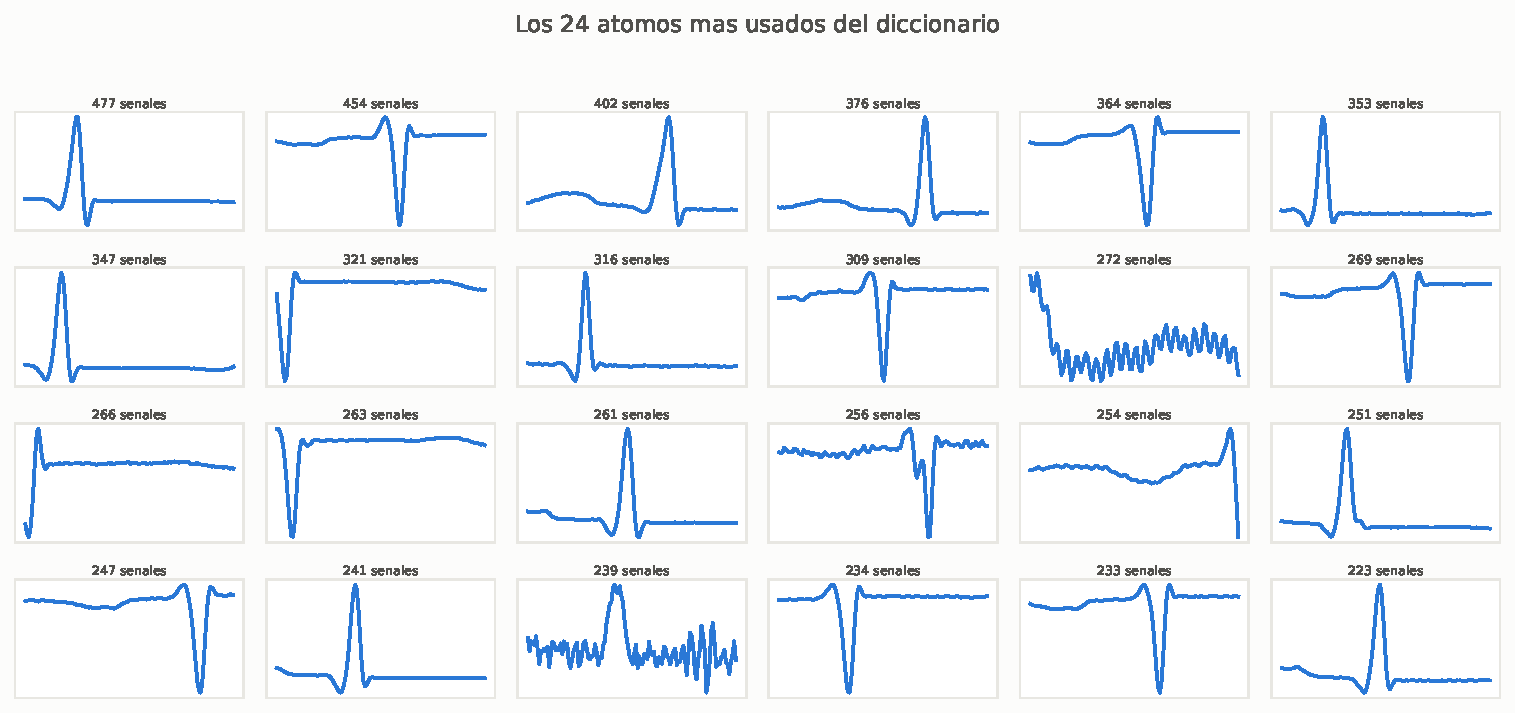
\includegraphics[width=0.8\linewidth]{atomos.pdf}
  \caption{Los átomos más usados del diccionario entrenado, con el
    número de ventanas de prueba en que participa cada uno. Son
    complejos QRS en distintas posiciones y polaridades.}
  \label{fig:atomos}
\end{figure}

Los átomos más usados (figura~\ref{fig:atomos}) son complejos QRS
desplazados dentro de la ventana y con ambas polaridades. El
diccionario no guardó ventanas sino la forma del latido en distintas
posiciones, que es lo que permite describir cualquier ventana con
pocos de ellos.

\subsection*{Original contra reconstrucción}

\begin{figure}[!t]
  \centering
  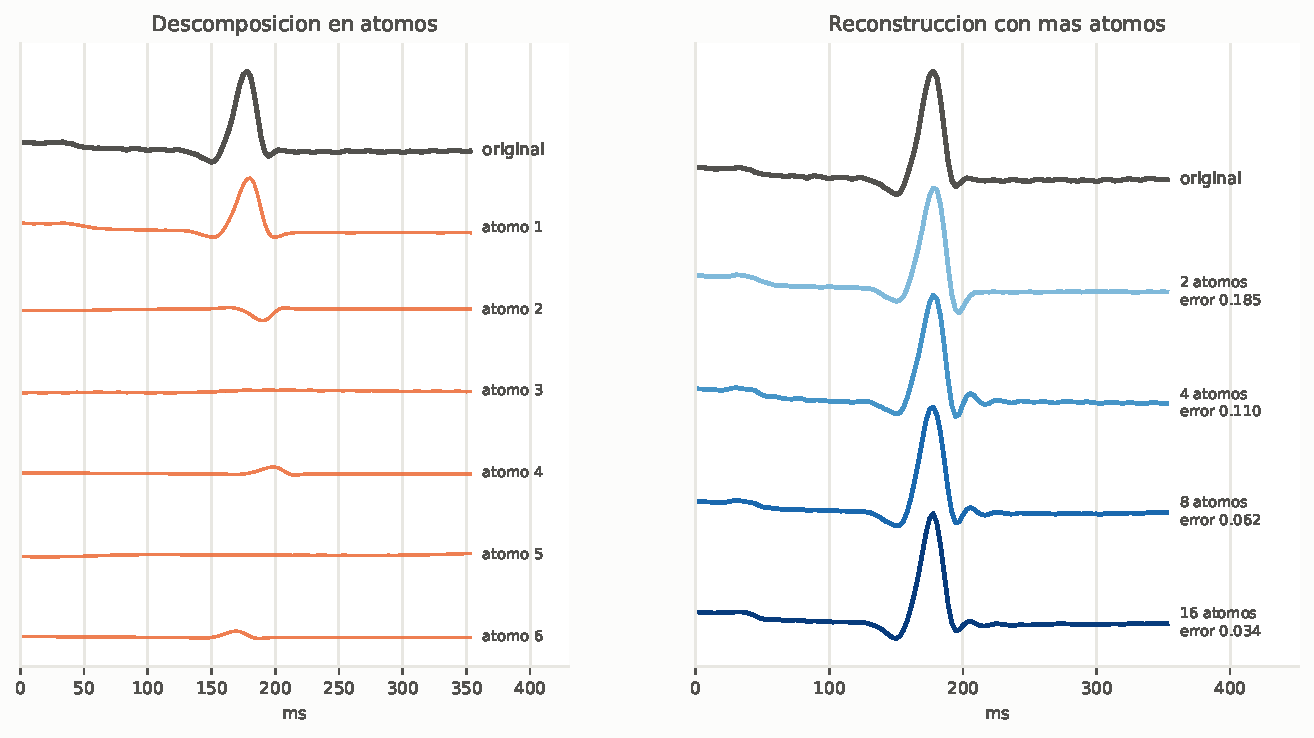
\includegraphics[width=0.9\linewidth]{reconstruccion.pdf}
  \caption{Una ventana de prueba con un latido completo. Izquierda: los
    primeros átomos en que se descompone. Derecha: su reconstrucción
    con 2, 4, 8 y 16 átomos, desplazada en vertical para que no se
    tape con la original.}
  \label{fig:reconstruccion}
\end{figure}

La figura~\ref{fig:reconstruccion} es la comparación que pide el
objetivo. El primer átomo que escoge OMP ya tiene la forma del QRS;
los siguientes corrigen detalles. El error baja de 0.185 con 2 átomos a
0.110 con 4, 0.062 con 8 y 0.034 con 16. Guardar la ventana con 9
átomos cuesta 9 coeficientes y 9 índices en lugar de 128 muestras.

\subsection*{Contra diccionarios que no aprendieron}

El error de 0.115 no dice mucho sin una referencia. Se comparó contra
dos diccionarios del mismo tamaño: $D_0$, las ventanas sin entrenar, y
una DCT sobrecompleta, el caso típico de diccionario fijo.

\begin{table}[H]
  \centering
  \begin{tabular}{rrrr}
    \toprule
    \textbf{Átomos} & \textbf{Aprendido} & \textbf{$D_0$}
      & \textbf{DCT} \\
    \midrule
     1 & \textbf{0.327} & 0.342 & 0.798 \\
     2 & \textbf{0.232} & 0.257 & 0.682 \\
     4 & \textbf{0.174} & 0.205 & 0.540 \\
     8 & \textbf{0.130} & 0.162 & 0.363 \\
    16 & \textbf{0.101} & 0.125 & 0.184 \\
    32 & 0.081 & 0.088 & \textbf{0.074} \\
    \bottomrule
  \end{tabular}
  \caption{Error relativo sobre las 2539 ventanas de prueba según el
    número de átomos permitidos. En negritas el menor de cada renglón.}
  \label{tab:diccionarios}
\end{table}

Con pocos átomos, que es el régimen que importa en una representación
dispersa, el diccionario aprendido gana en todos los casos: con 8
átomos tiene un 20\,\% menos de error que $D_0$ y la tercera parte que
la DCT. Que $D_0$ quede tan cerca muestra que tomar ventanas reales ya
es un buen punto de partida, y lo que agrega K-SVD es ajustarlas.

Con 32 átomos la DCT termina ganando. La explicación probable es que
el diccionario aprendido se especializó en la forma del latido, y lo
que queda sin explicar después de muchos átomos es ruido de alta
frecuencia, que los cosenos representan mejor. No se verificó
directamente, pero es consistente con que la DCT mejore mucho más
rápido que los otros dos al pasar de 16 a 32 átomos.

\subsection*{Otros pacientes}

\begin{figure}[H]
  \centering
  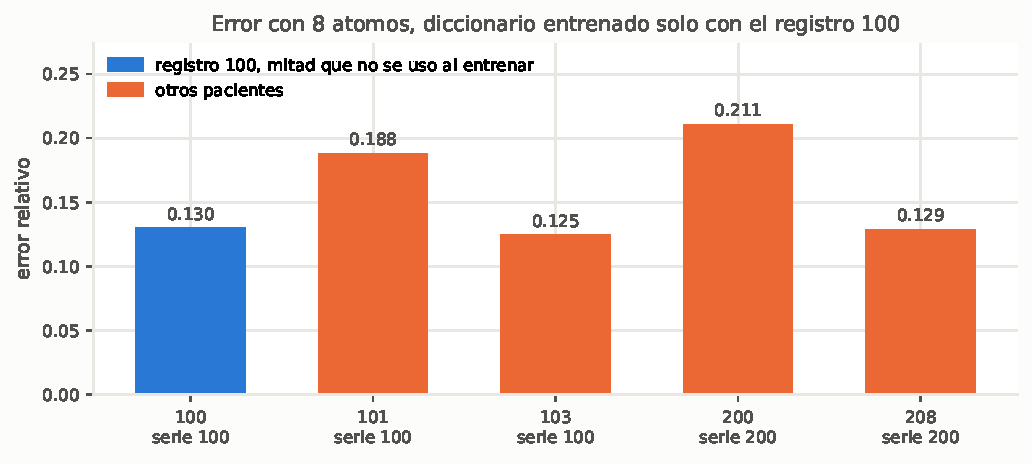
\includegraphics[width=0.75\linewidth]{pacientes.pdf}
  \caption{Error con 8 átomos en cada paciente, usando el diccionario
    entrenado solo con el registro 100.}
  \label{fig:pacientes}
\end{figure}

El diccionario del registro 100 se aplicó sin reentrenar a otros
cuatro pacientes (figura~\ref{fig:pacientes}). En los registros 103 y
208 el error es igual o menor que en la propia mitad de prueba del
100, y en 101 y 200 sube a 0.188 y 0.211, que se traduce en 11.5 y
12.6 átomos para llegar al umbral en lugar de 9.5. La serie no
predice el resultado: el 208, de la serie de arritmias, se reconstruye
tan bien como el 100, y el 101, de la misma serie que el 100, no. Un
diccionario de un solo paciente cubre las morfologías parecidas a la
suya pero no todas, y el siguiente paso natural es entrenar con varios
pacientes, opción que ya admite la implementación.

\section{Conclusiones}

K-SVD aprendió un diccionario cuyos átomos son la forma del latido, y
con él una ventana de 128 muestras se reconstruye al 10\,\% de error
con unos 9 coeficientes. La ventaja sobre un diccionario fijo es
grande precisamente donde importa, con pocos átomos, y desaparece
cuando se permiten muchos. La SVD aparece como la solución exacta del
paso de actualización: cada átomo es la mejor aproximación de rango 1
de lo que le toca explicar.

\section*{Referencias}

\begin{enumerate}[label={[\arabic*]}, itemsep=0.1em, leftmargin=*]
  \small
  \item M. Aharon, M. Elad y A. Bruckstein, \emph{K-SVD: An algorithm
        for designing overcomplete dictionaries for sparse
        representation}, IEEE Transactions on Signal Processing,
        54(11), 4311-4322, 2006.
  \item Y. C. Pati, R. Rezaiifar y P. S. Krishnaprasad,
        \emph{Orthogonal matching pursuit: recursive function
        approximation with applications to wavelet decomposition},
        27th Asilomar Conference on Signals, Systems and Computers,
        40-44, 1993.
  \item C. Eckart y G. Young, \emph{The approximation of one matrix by
        another of lower rank}, Psychometrika, 1(3), 211-218, 1936.
  \item G. B. Moody y R. G. Mark, \emph{The impact of the MIT-BIH
        Arrhythmia Database}, IEEE Engineering in Medicine and Biology
        Magazine, 20(3), 45-50, 2001.
  \item A. L. Goldberger et al., \emph{PhysioBank, PhysioToolkit, and
        PhysioNet}, Circulation, 101(23), e215-e220, 2000.
  \item Visual Kernel, \emph{SEE Matrix}, serie de videos en YouTube
        sobre matrices, descomposición espectral y SVD.\\
  \url{https://www.youtube.com/playlist?list=PLWhu9osGd2dB9uMG5gKBARmk73oHUUQZS}
\end{enumerate}

\end{document}

%############################# END OF REPORTE.TEX ##############################
%###############################################################################
